\documentclass[a4,center,fleqn]{NAR}
\UseRawInputEncoding
\usepackage{siunitx}
\usepackage{hyperref}
\hypersetup{
    colorlinks=true,
    linkcolor=blue,
    filecolor=magenta,      
    urlcolor=cyan,
} 
\urlstyle{same}
\usepackage{graphicx}%graphic path
\graphicspath{{./figs/}}%graphic path
\usepackage{epstopdf}
% Enter dates of publication
\copyrightyear{2008}
\pubdate{31 July 2009}
\pubyear{2009}
\jvolume{37}
\jissue{12}

%\articlesubtype{This is the article type (optional)}

\begin{document}

\title{Seasonal Anti-cyclonic Vortex Event Reveals Connections between Environmental Features and Oligotrophic Oceanic Virio- and Bacterioplankton Communities}

\author{%
K. Eric Wommack\,$^{1,*}$,
Ling-yi Wu\,$^{2}$,
Gonçalo J. Piedade\\,$^{3}$,
Ana M. Martins\,$^{4}$,
Kay D. Bidle\,$^{5}$%
and Shawn Polson\,$^{1}$%
\footnote{To whom correspondence should be addressed.
Tel: +01 302-831-4362; Fax: +44 000 0000000; Email: wommack@dbi.udel.edu; wommack@udel.edu}}

\address{%
$^{1}$Center for Bioinformatics and Computational Biology, University of Delaware, 15 Innovation Way, Newark, DE, 19711, United States,
$^{2}$Department of Water Science and Policy, College of Agriculture and Natural Resources, University of Delaware, Newark, DE,  19716, United States,
$^{3}$Department of Marine Microbiology, NIOZ Royal Netherlands Institute for Sea Research, Den Burg, Texel, 1790 AB , Netherlands,
$^{4}$Department of Oceanography and Fisheries, University of the Azores, Ponta Delgada, Regiao Autonoma dos Acores, Portugal and
$^{5}$Department of Marine and Coastal Sciences, Rutgers University, 71 Dudley Rd., New Brunswick, NJ, 08901, United States}
% Affiliation must include:
% Department name, institution name, full road and district address,
% state, Zip or postal code, country

\history{%
Received January 1, 2009;
Revised February 1, 2009;
Accepted March 1, 2009}

\maketitle

\begin{abstract}
Test branch
This my edit 2.
This is my edit
I added one line.
I am testing the editing functions in GitHub.
Virioplankton are major players within oceanic ecosystems, impacting biogeochemical cycling of nutrients and energy.
Virioplankton can only reproduce themselves through host infection, mostly bacterioplankton, and thus influence marine ecosystems through interactions with bacterioplankton.
Observations of temporal and spatial variations in viral and bacterial communities are important for understanding the patterns of aquatic microbial diversity and how these changes may affect ocean biogeochemical processes.
This study focuses on characterizing the patterns of marine viral and bacterial diversity in the pelagic and oligotrophic ocean.
Seawater down to 75 meters was collected from a fixed station off Faial Island (station SCFP) during late spring and summer of 2016.
Virioplankton and bacterioplankton communities were characterized using Ribonucleotide triphosphate reductase (RTPR) and 16S rDNA amplicon sequences, respectively.
RTPR is one of the most abundant ribonucleotide reductase (RNR) genes, carried mostly by lytic viruses.                                           
We studied the dynamics of this group in conjunction with the co-occurring bacterial community at one location in order to (a) contextualize observations of virioplankton community composition and diversity in environmental changes and microbial abundances, (b) investigate beta and alpha diversity of virioplankton and  bacterioplankton communities across the sampling days and sampling depths and compare their patterns, (c) investigate seasonal and spatial dynamics of distinct RTPR-carrying viruses and bacteria populations, (d) detect statistical associations between distinct viruses and bacteria populations to understand how viruses and bacteria community may influence each other and determine potential phage-host relationships.
Statistics methods and bioinformatics tools that account for the compositional characteristics of hight-throughput sequencing (HTS) datasets are used to overcome challenges brought by biases that are inherent to HTS datasets derived from environmental samples.
We found that seasonal anti-cyclonic vortex, which causes water stratificication accompanying with temperature and other environmental changes, influenced bacterioplankton community diversity, and subsequently influenced changes in virioplankton community diversity. 
Among the multitude of discovered virioplankton and bacterioplankton populations, only a few populations appear to be most responsible for changes in thier community diversity.
Close correlations are found between viruses from the same phylogenetic clades and bacteria from the same order indicated that phylogenetically similar viruses or bacteria thrive in similar environments.
\end{abstract}


\section{Introduction}

Virioplankton are major players in ocean ecosystems, impacting biogeochemical cycles of nutrient elements and energy (\cite{Suttle2005}). 
Viruses are the most abundant biological entities on Earth. 
The number of viruses has been estimated to be on the order of 10\textsuperscript{31} individuals, which is roughly about one billion times the number of stars in the observable universe (10\textsuperscript{22}) (\cite{Hatfull2006}). 
Viruses cannot reproduce by themselves. They depend on their host’s machinery to replicate the viral genome and produce viral proteins to make new capsids (\cite{Whittaker1998}; \cite{Doms1993}). 
The hosts of virioplankton are mainly bacterioplankton. Thus, the behaviors of virioplankton populations influence the lives of bacterioplankton. 

Virioplankton in lytic cycles can kill bacterioplankton through viral lysis. 
The mortality of bacterioplankton caused by viral lysis is one of the major top-down controls on 

% **************************************************************
% Keep this command to avoid text of first page running into the
% first page footnotes
\enlargethispage{-65.1pt}
% **************************************************************
bacterioplankton productivity – it is responsible for 10 to 40\% of the mortality rate of the bacterial community (\cite{Fuhrman1999}). 
Nutrients inside of the bacterioplankton cells are released into the environment after viral lysis and thus contribute to nutrient pools within marine ecosystems. 
Bacterioplankton lysis comprises the largest carbon flux process between biomass and dissolved organic matter (DOM) on the globe (150 gigatons of C/yr) (\cite{Wilhelm1999}; \cite{Suttle2005}).  
The conversion of biomass to DOM performed by viral lysis is five times more common than that performed by other biological mechanisms (\cite{Wilhelm1999}; \cite{Suttle2005}). 
The flux from biomass to DOM sustains the cycles of nutrients, such as carbon, nitrogen, phosphate, iron and etc., which are reused by living bacterioplankton and other organisms.
 The availability and limitation of different nutrients manipulates the bacterioplankton populations through bottom-up control (\cite{Wilhelm1999}; \cite{Suttle2005}). 
 Besides shaping the composition and diversity of marine bacterial communities through top-down and bottom-up controls, viruses can influence bacterial behaviors (such as improving fitness in the face of  environmental changes ((\cite{Jiang1998}); (\cite{Schwartz:2017aa})) and altered metabolic pathways((\cite{Ochman2000});\cite{Rosenwasser2016})) through horizontal gene transfer and expression of auxiliary metabolic genes (AMGs) during viral infection. 
  
In summary, virioplankton plays a key role in marine ecosystems mainly through the interactions with their host bacterioplankton. 
Different virioplankton populations can shape the ecology and evolution of host populations in unique ways. 
However, the behavior of individual virioplankton populations and the detailed interaction between specific virioplankton and bacterioplankton populations remain largely unknown. 
This study focuses on characterizing the patterns of marine microbial diversity in pelagic ocean to acquire a better understanding of marine ecosystems. 
Diversity of virioplankton communities are expected to dynamically respond to environmental changes and bacterioplankton communities.

The 16S rRNA gene has proven to be a robust marker gene to comprehensively characterize community structure and diversity of bacterioplankton from the environment. 
This is largely because the 16S rRNA gene is found in all bacterial species.  
However, the virioplankton lacks a universal marker gene because of the polyphyletic nature of viral evolution. 
There is no single viral gene existing in all of the virioplankton. 
However, a few genes are widespread across a number of viral populations and thus can be used as marker genes to characterize the diversity of a subset of virioplankton in the environment, such as DNA polymerase A gene (encoding DNA polymerase I) (\cite{Schmidt2014}), major capsid protein gp20 gene (\cite{Zhong2002}), major capsid protein gp23 gene (\cite{Comeau2008}) and Ribonucleotide Reductase (RNR) genes (\cite{Sakowski2014}). 
DNA Polymerase I is an essential protein for DNA replication and repair in prokaryotes and is found in many tailed bacteriophages. 
Gp20 and gp23 are structural proteins of tailed Myoviruses.
RNR is an enzyme that catalyzes the formation of deoxyribonucleotides from ribonucleotides, thus prime DNA synthesis (\cite{ELLEDGE1992119}).


RNR genes are promising marker genes to characterize viral diversity (\cite{Sakowski2014}) because they are functionally non-redundant, abundant and widely distributed among marine viruses. 
RNRs are the only known enzymes able to reduce ribonucleotides to deoxyribonucleotides, a key step for DNA synthesis (\cite{Lundin2010}; \cite{ELLEDGE1992119}). 
\textbf{Thus, RNRs are vital to nucleotide biosynthesis, under rigorous evolutionary selection pressure, and among the most abundant annotated genes in marine virome libraries (\cite{Dwivedi2013}). 
Importantly, RNR genes are present in all three families of tailed phages in the order Caudovirales and have been identified in viruses infecting hosts within all three domains of life.}
Lytic viruses usually carry RNRs so that they can synthesize DNA and replicate fast by ensuring a steady supply of deoxyribonucleotides for DNA synthesis (\cite{Sullivan2005}). 
Therefore, RNRs are  representative of many lytic marine phages, which significantly influence nutrient cycles within the ocean (\cite{Brussaard2008}). 
 
In addition, RNRs are biologically informative and form three physiological classes according to reactivity with oxygen. 
Class I RNRs are oxygen-dependent. 
Class II RNRs are oxygen-independent and rely upon an adenosylcobalamin (vitamin B12) co-factor for ribonucleotide reduction. 
Class III RNRs are sensitive to oxygen. 
Class I and Class II RNRs, not Class III RNRs, are expected to be present in the surface water of pelagic ocean because of the abundance of oxygen (\cite{Nordlund2006}). 
Ribonucleotide triphosphate reductase (RTPR) reduce ribonucleotide triphosphate to deoxyribonucleotide triphosphate.
Among all of the clades of known RNRs, RTPR RNRs were the most abundant RNR clade in studied viromes, with an estimated 34 to 54\% of all RNR-carrying viruses carrying a RTPR RNR gene (\cite{Sakowski2014}). 
Degenerated RTPR primers developed by Sakowski were used in the study to amplify RTPR genes (\cite{Sakowski2014}).

Thanks to the advancement of sequencing techniques, second-and third- generation sequencing technologies can now provide massive amounts of sequencing data to characterize the diversity of viral and microbial communities. 
However, the traditional ways to analyze sequencing data, such as rarefaction, Bray-Curtis similarity matrix,  principal coordinates analysis (PCoA) and correlation tests, are problematic (\cite{McMurdie2014}; \cite{Weiss:2017aa}). 
These methods treat the sequencing data as ecological data where the counts of reads assigned to organisms are often normalized to a constant area or volume. 

In a typical ecological study it is possible that different species co-exist, and the presence of one individual of one species does not influence the ability to detect the presence of another individual from another species. 
For example, an ecological survey intends to count the numbers of tigers and the numbers of ladybugs in a certain area. 
The numbers of total counts of tigers and ladybugs are not fixed, and the numbers of tigers are not correlated to the numbers of ladybugs during the survey (\cite{Gloor2017}). 

In contrast, datasets collected by high-throughput sequencing (HTS) are compositional because the numbers of sequences obtained from a sample have an arbitrary maximum imposed by the instrument (\cite{Gloor2017}). 
Compositional data consist of vectors whose components are the proportion or percentages of some whole. 
The peculiarity of compositional data is that their sum is constrained to be some constant, equal to 1 for proportions, 100 for percentages or possibly some other constant c for other situations such as parts per million (ppm) in trace element compositions (\cite{10.2307/2345821}). 

As for sequencing, an Illumina MiSeq sequencer can generate 25 million reads per run at maximum. 
Pacbio RSII sequencer can generate about a million reads per SMRT-cell at maximum and Pacbio Sequel sequencer can generate up to seven million reads per unit instrument run. 
Since the total read counts observed in an HTS run is fixed, the read counts gained for a certain composition (bacterioplankton or virioplankton population in this case) from a sample are influenced by the read counts gained for other compositions from the same sample or from other samples. 


Moreover, bias is inherent to HTS datasets derived from environmental samples as each step in the experimental workflow preferentially detects some taxa over others (\cite{Brooks:2015aa}; \cite{Sinha:2017aa}, \cite{BROOKS2016336}). 
As a result, the measured relative abundances of each population within the sample can be systematically distorted from their true values. 
Bias can lead to qualitatively incorrect conclusions about differential relative abundance, compositional similarities, and correlations between different compositions from environmental samples.
Both of the absolute and relative read counts are irrelevant and cannot be used to interpret microbial diversity (\cite{Gloor2017}).
Recent studies found that analyses based on proportions between compositions from different samples are less sensitive to bias than analyses based on relative abundance of each composition, which emphasizes the importance of using compositional data analysis tools to analyze HTS datasets derived from microbial/viral studies (\cite{McLaren2019}).

Overall, HTS datasets derived from viral or microbial studies are compositional and should be treated as compositional data at all stages of analysis. 
Thus, we used statistics analysis methods designed for compositional data to analyze the sequencing dataset. 
To date, compositional data analysis paradigms have been applied to the study of human microbiomes (\cite{Bian2017}) but have not been widely used in biogeography studies of marine viruses and microbes. 


\section{MATERIALS AND METHODS}

\subsection{Study Site and Sample Collection}

Seawater was collected from the South of the Channel Faial-Pico (SCFP) Island, Azores, Portugal at 0 m, 5 m, 25 m, 50 m and 75 m depths on April 14th, May 12th, June 8th, June 22nd, July 11th, July 27th, August 5th and September 8th, 2016 (Julian Day: 103, 132, 159, 173, 192, 208, 217 and 251). 
SCFP is one of the islands in the Azores archipelago in Northeastern Atlantic, located at 38 \degree23'11.67"N and 28 \degree35'6.14"W, 8.6 nautical miles off Horta city (Faial island) and 6.4 nautical miles off São Mateus (Pico island).

Surface seawater was collected by submerging a 22 liter carboy into the water directly.
Seawater at other depths was collected by sending a 2.5 liter Niskin bottle to each depth for three times and transfer all the water from the same depth to a 5 liter carboy.
All containers (including carboys and bottles) were washed using deionized water, followed by 0.1 M HCl rinse and deionized water rinse at the laboratory before sampling. 
\textbf{Containers were washed twice with seawater at the sampling site just before collecting seawater.
More details here.}

In addition, a MIDAS CTD profiler (Valeport, Totnes, United Kingdon) was used to measure, \textbf{in triplicate}: the water temperature (\degree C), salinity (SPC), current direction (\degree), and current velocity (m/s).
Temperature and salinity data from the CTD profiler were visualized using Ocean Data View (\url{https://odv.awi.de}). 
Temperature and salinity data between sampling days were extrapolated using the weighted average grid method (\cite{Schlitzer2002}).
Chlorophyll \textit{a}, sea surface temperature, particulate organic carbon, particulate inorganic carbon and photosynthetically available radiance data in the year of 2016 were accessed from the NASA Ocean Color website (http://oceancolor.gsfc.nasa.gov/) at 1 km resolution. 
The Level 2 data was calculated using SeaDAS 7 for the nine km\textsuperscript{2} area around the sampling station SCFP (Figure~supplementary figure1). 
Data was extracted using the pixel extraction tool. 
The average values of each day and month were calculated in Excel. 
The “Minimum-Maximum Normalization” (equation~\ref{equation1}) method was performed on the data to improve data visualization (\cite{Larose2014}). 
x\textsubscript{i} is the value of the i\textsubscript{th} data from dataset x. min(x) is the minimum of dataset x and max(x) is the maximum of dataset x. z\textsubscript{i} is the normalized value of data x\textsubscript{i}.

\begin{equation}
  z_{i}(\%)=\frac{x_{i}-\min (x)}{\max (x)-\min (x)} \times 100
  \label{equation1}
\end{equation}


\subsection{Sample Preparation}

Two mL of seawater was fixed with 0.5\% glutaraldehyde and collected into 5 mL vials for flow cytometry analysis.
Two hundred and fifty mL of seawater was fixed with 0.4\% formalin and collected into a 1 L dark bottle for phytoplankton identification and enumeration.
Seawater samples were transported to the laboratory as quickly as possible for further processing. 
Seawater for pigment analyses was filtered onto GF/F glassfiber filters (\SI{0.7}{\micro\metre} pore-size, 25 mm diameter), dried with absorbent paper, and stored at -80 \degree C. 
Samples for pigments and phytoplankton counts are still waiting further processing

Viral and microbial fractions were separated through peristaltic filtration.
Each water sample was filtered sequentially through a \SI{0.22}{\micro\metre} pore-size Sterivex filter (Milipore, SVGP01050) followed by a \SI{0.02}{\micro\metre} pore-size Anotop filter (Whatman, WHA68092002) (Steward and Culley, 2010; Mueller, Culley and Steward, 2014a).
Filtration through the \SI{0.22}{\micro\metre} pore-size Sterivex filters was performed using a vacuum pump (Milipore, SD1P014M04). 
Filtration through the \SI{0.02}{\micro\metre} pore-size Anotop filters was performed using a fabricated calking gun, which generated even and steady pressure for water filtration.
After filtration, both filters (\SI{0.22}{\micro\metre} and \SI{0.02}{\micro\metre}) were sealed and stored at -80\degree C until DNA extraction. 

\subsection{Microbial and Viral Abundances}

Place Holder for Goncalo

\subsection{Viral DNA Extraction and Tag-Encoded RTPR Amplicon Sequencing}

For the viral RTPR gene analysis, DNA was extracted from \textbf{\SI{500}{\micro\liter}} of the treated viral concentrate using the MasterPure complete DNA/RNA purification kit (Epicentre,  Madison, WI, United States) per the manufacturer’s instructions with adaptions and quantified with a HS DNA Qubit fluorescent concentration assay, described in detail in the Supplementary1. 
For each sample, DNA was used in the initial amplification PCR with 35 cycles, followed by 22 cycles of limited PCR using distinctive barcodes designed in Wommack Lab. 
The final libraries were then quantitated by KAPA SYBR FAST qPCR kit and sequenced on the PacBio RSII (Pacific Biosciences, Menlo Park, CA, United States).

\subsection{Bacterial DNA Extraction and Tag-Encoded 16S Amplicon Sequencing}

For the bacterial 16S rDNA gene analysis, DNA was extracted from each of the \SI{0.22}{\micro\meter} filters utilizing an adapted phenol/chloroform method  (\cite{Diez2001}) described in detail in the Supplementary1.
The V3-V4 hypervariable region of the 16S rRNA gene was PCR-amplified and sequenced on the Illumina MiSeq (Illumina, San Diego, CA, United States) utilizing a dual-indexing strategy for multiplexed sequencing developed at the Institute for Genome Sciences for twice (Fadrosh et al., 2014), described in detail in the Supplementary2. 
Obtained bacterial 16S rDNA gene amplicon sequences from the two libraries were analyzed individually for core diversity, described in detail in Supplementary2.
The results showed that the two datasets are similar to each other.
Thus, obtained bacterial 16S rDNA gene amplicon sequences from the two libraries were combined together for downstream analysis.

\subsection{Virioplankton RTPR Gene Data Analysis}

RTPR gene reads from virioplankton were initially screened for low quality bases and short or long read lengths at PacBio Data Repository of Delaware Biotechnology Institute (\url{http://pacifica.dbi.udel.edu}). 
Circular consensus sequences were generated. 
Reads with less than three full passes, less than 98\% of minimum predicted accuracy and with a length shorter than 250 bp or larger than 5000 bp were excluded. 
Generated circular consensus sequences were demultiplexed using split\textunderscore libraries.py command from QIIME1. 
Barcode-demultiplexed reads were screened for forward and reverse degenerate primer sequences using Daniel Nasko’s demultiplex.pl script (\url{https://github.com/dnasko/biobin/tree/master/pcr_products/adapter_searching}). 

Reads containing both forward and reverse primer sequences with at least 85\% of similarity on their first 60 base pairs were retained.
Barcode and primer sequences were trimmed from the reads.
Barcode-primer-demultiplexed reads were translated into amino acid sequences and the frame shifts were corrected using Daniel Nasko’s frameshift polisher script (\url{https://github.com/dnasko/frameshift_polisher}). 
RTPR amino acid sequences from rnrdb (\cite{Lundin:2009aa}) and Tara Ocean (\cite{Pesant:2015aa}) databases were used as references.
Translated RTPR amino acid sequences were screened for key catalytic sites using Protein active site validator (PASV) designed by Ryan Moore (\url{https://github.com/mooreryan/pasv}).
An RTPR amino acid sequence with all of the active key residues indicates a functional RTPR. 
RTPR Amino acid sequences with key residues C439, E441 and C46 (\textit{E. coli} numbering) were were aligned using the FFT-NS-1 algorithm in MAFFT alignment (\cite{Katoh2002}) in Geneious 10.0.9 (\url{https://www.geneious.com}) and trimmed to the region of interest (H23 to C783 in \textit{E. coli}).
Quality-controlled RTPR amino acid sequences were clustered at 95\% \textit{de novo} into operational taxonomic units (OTUs) using \texttt{cluster\textunderscore fast} command in USEARCH (\cite{Edgar2010}). 
OTUs occurring no more than twice among all samples were removed.

Beta diversity was determined through principal component analysis (PCA) plots of Aitchison distances between samples calculated using the R package compositions (\cite{compositions}) and tested for significance with \texttt{beta-group-significance} command (\cite{Anderson:2001aa}) in QIIME2.
It should be noted that zero count OTUs were replaced by an imputed value using the count zero multiplicative method from the zCompositions R package (\cite{Palarea-Albaladejo:2015aa}). 
The centered log ratio (clr) transform was applied to the zero replaced data set, and the data were subsequently used as input for a singular value decomposition (SVD). This approach returns data where the samples are separated by the variance in the OTUs rather than by differences in abundant OTUs (\cite{Gloor2016}; \cite{Gloor2016_2}). 

The dendrogram of virioplankton samples was made based on Aitchison distances between samples using Hierarchical Cluster Analysis in the R package stats  (\cite{R})and visualized using Iroki (\cite{Moore2018}).
Correlations between virioplankton diversity and associated metadata, such as environmental features, microbial abundances and viral abundance, was tested using Mantel test  (\cite{Mantel1967};\cite{Pearson1895};\cite{Spearman2010};) in QIIME2.
Associated metadata sets that have significant correlations with virioplankton diversity (p-value < 0.05) were plotted next to the dendrogram of virioplankton samples using Iroki (\cite{Moore2018}).

Alpha diversity was calculated using the R packages: DivNet (\cite{Willis305045}), breakaway (\cite{Willis:2015aa}), phyloseq (\cite{McMurdie:2013aa}), tidyverse (\cite{tidyverse}) and ggplot2 (\cite{ggplot2}) on raw viral RTPR OTU table and tested for significance using betta function in R package breakaway (\cite{Willis:2017aa}).
Estimated Shannon indices and Estimated Simpson indices were converted to Hill numbers for better visualisation (\cite{Kang:2016ab}).

Correlation analysis were performed on samples from the same depth.
Three pseudo-replicates were generated for each sample.
Correlation analyses were done using a symmetric modification of the 􏰓 metric (\cite{propr}), which measures the variance in the ratios between OTUs. OTUs with a low ratio variance are said to be compositionally associated. The 􏰓 metric (\cite{metric}) was calculated as an expected value across clr-transformed Monte Carlo Dirichlet replicates (\cite{propr}; \cite{Fernandes}) generated by the aldex.clr function , and values of 􏰏0.65 were taken as indicating association between pairs of OTUs.

Differential abundance analysis were performed on samples from the same depth on from the same day.

\subsection{Bacterioplankton 16S rDNA Gene Data Analysis}

16S rDNA gene reads were initially screened for low quality bases and short read lengths (Fadrosh et al., 2014), paired reads were merged using PANDAseq (Masella et al., 2012), de- multiplexed, trimmed of artificial barcodes and primers, and assessed for chimeras using UCHIME in de novo mode, as implemented in Quantitative Insights Into Microbial Ecology (QIIME; version 1.9.1-20150604) (Caporaso et al., 2010). Quality- controlled reads were clustered at 97\% de novo into operational taxonomic units (OTUs) with the SILVA 16S database (Quast et al., 2012) in QIIME (Caporaso et al., 2010). All sequences taxonomically assigned to chloroplasts were removed from further downstream analysis. When appropriate, data was normalized using metagenomeSeq’s cumulative sum scaling to account for uneven sampling depth (Paulson et al., 2013b).
To visualize the relative abundance of bacterial phyla, stacked bar charts were generated using ggplot2 (Wickham, 2009). In addition, bacterial taxa were summarized at the genera level in QIIME (level = 6) and those with a maximum relative abundance greater than 1\% in at least one sample were used to build a heatmap via R (ver. 3.3.2) and vegan heatplus (Ploner, 2012).
Significance tests were conducted using a Tukey’s HSD Test between filter size fractions and among sampling dates. Additionally, Pearson correlation coefficients were calculated to identify associations between the water characteristics and the relative abundance of the bacterial phyla/genera.
Alpha diversity was calculated using the R packages: Bioconductor (Huber et al., 2015), metagenomeSeq (Paulson et al., 2013a), vegan (Oksanen et al., 2007), phyloseq (McMurdie and Holmes, 2013), fossil (Vavrek, 2011), biomformat (McMurdie and Paulson, 2016), and ggplot2 (Wickham, 2009) on data rarefied to an even sampling depth (55,307 sequences) and tested for significance using a Tukey’s HSD Test.
Beta diversity was determined through principle coordinates analysis (PCoA) plots of Bray–Curtis, Weighted and Unweighted UniFrac distances calculated using the R package phyloseq and tested for significance with ANOSIM (9,999 permutations) (Beals, 1984; Clarke, 1993; Lozupone et al., 2011; McMurdie and Holmes, 2013).

\section{RESULTS}

\subsection{Seawater Characteristics}

\begin{figure*}[t]
\begin{center}
\includegraphics[width=15cm]{watercolumn}
\end{center}
\caption{CTD-derived vertical profile contours of  \textbf{(A)} temperature , \textbf{(B)} salinity at station SCFP from May12 to Aug05 in 2016.
}
\label{watercolumn}
\end{figure*}

Temperature and salinity of surface seawater were homogeneous prior to June, especially in the upper 40 m of the water column, indicating seawater was well-mixed in the beginning of sampling period (Figure~\ref{watercolumn}).
Temperature started to increase in early June, continuing throughout the summer. 
Coincidently, salinity increased slightly with a distinct increase centered at 75 m depth, especially on Jul11.  
The stratification patterns of temperature and salinity suggested the presence of a downwelling anticyclonic vortex in the region. 
Downwelling anticyclonic vortex is likely to prevent nutrient from deeper and colder seawater from coming up to the sea surface, causing nutrient depletion in the region.
Salinity tended to be homogeneous again on the surface seawater in August, potentially indicating an upwelling vortex from the deep ocean to the surface water.
The upwelling vortex is likely to bring nutrient from deeper and colder seawater to the sea surface and supply nutrient for the food web.
Unfortunately, temperature and salinity profile data is missing for the last sampling day due to equipment failure. 
The stratification intensity was assumed to mitigate according to data from similar studies in nearby areas \textbf{(need to confirm)}.

\subsection{Bacterial 16S rDNA Gene and Viral RTPR Gene Sequencing Effort}
In total, 35 bacterioplanton samples were PCR-amplified for the 16S rDNA gene and sequenced. 
After sequence quality filtering, 1,779 ASVs were identified from a total of 0.9 million sequences across all samples, with an average number of ca. 26,251 sequences per sample and an average of ca. 281 ASVs.

29 virioplankton samples were PCR-amplified for the 16S rDNA gene and sequenced.
Amplification was failed in six of the virioplankton samples.  
After sequence quality filtering, 220 OTUs (95\% identity) were identified from a total of 30 thousand sequences across all samples, with an average number of ca. 1,034 sequences per sample and an average of ca. 87 OTUs.

\subsection{Bacterial and Virioplankton Community Composition and Temporal Variations}

The most abundant bacterioplankton phyla were Proteobacteria,  Bacteroidetes and Cyanobacteria in all samples as order using CLR transformed abundance (Supplementary Table S1), however, the most abundant bacterioplankton phyla were Proteobacteria, Cyanobacteria and Bacteroidetes in all samples as order using relative abundance (Supplementary Table S2).

\subsection{Bacterioplankton and Virioplankton Beta Diversity}

\begin{figure*}[t]
\begin{center}
\includegraphics[width=15cm]{sample_day_pca}
\end{center}
\caption{(A) bacterioplankton and (B) virioplankton responded similarly to sampling days.
}
\label{bata_div}
\end{figure*}

Beta diversity comparisons using PCA plots of Aitchison distances computed for all samples revealed obvious clustering before (excluding) and after (including) sampling day Jun22 along PC1 and PC2, which accounted for nearly 38\%  and 37\% of the variation of bacteriolankton and virioplankton, respectively.
For both bacterioplankton and virioplankton, samples collected before Jun22 clustered together on the left part of PC1 while samples collected after Jun22 clustered together on the middle-bottom part of PC2.
The clustering was significant for all the bacterioplankton samples taken from May12 and some of the bacterioplankton samples taken from Jun8 with both p and q value < 0.05 (Supplementary Table S3).
The clustering is not significant for any virioplankton samples (Supplementary Table S3).

Obvious clustering was also revealed across different sampling depths for bacterioplankton (Supplementary Figure S1A and Table S4). 
Samples clustered from 0 m depth distributed along the diagnol of the PCA plot.
Sample clustering shifted to the left and bottom of the PCA plot gradually as the depth went deeper.
All samples collected from 75 m depth clustered together on the left of PC1 and on the bottom of PC2 except for sample May12\textunderscore75m. 
No obvious clustering was seen across different sampling depths for virioplankton (Supplementary Figure S1B and Table S4).

\subsection{Relationships between Water Characteristics and Bacterioplankton or Virioplankton Beta Diversity}

\begin{figure*}[t]
\begin{center}
\includegraphics[width=13cm]{dendrogram_vertical}
\end{center}
\caption{(A) bacterioplankton and (B) virioplankton composition similarity dendrogram with associated environmental features. Average-linkage hierarchical clustering based on sample RTPR compositions.  Branch color is based on a scaled, 1-dimensional projection of sampling depths, sampling days, temperature and salinity onto the cubehelix color gradient.  Samples that are more similar to each other in color represent those that are more similar to each other with respect to the environmental parameters in the ordination.  The first bar series (blues) represents sampling depths (m), the second bar series (oranges) represent sampling days, the third bar series (red/orange) represents temperature (°C) and the forth bar series (purples) represents salinity (PSU).  Shorter bars and lighter colors indicate lower values, and longer bars with darker colors indicate higher values.
}
\label{dendrogram} 
\end{figure*}

Mantel test between sample composition similarity matrix and all metadata matrices showed that a few environmental features are correlated with sample compositions.
Sample dendrogram based on Aitchison distance between sample compositions were plotted against associated environmental features (Figure~ \ref{dendrogram}).

Temperature was the best indicator of sample composition similarity of both bacterioplankton (Spearman: r = 0.5, p = 0.001; Pearson: r = 0.53, p = 0.001) and virioplankton (Spearman: r = 0.32, p = 0.001; Pearson: r = 0.34, p = 0.001) communities among all the tested parameters (Supplementary Table S5).
Besides, sampling day and sampling depth were associated with sample compositions of both bacterioplankton and virioplakon communities.
Salinity was associated with bacterioplankton composition similarity.
No association was found between composition similarity and any microbial or viral abundance similarities.

\subsection{Bacterioplankton and Virioplankton Alpha Diversity}

\begin{figure*}[t]
\begin{center}
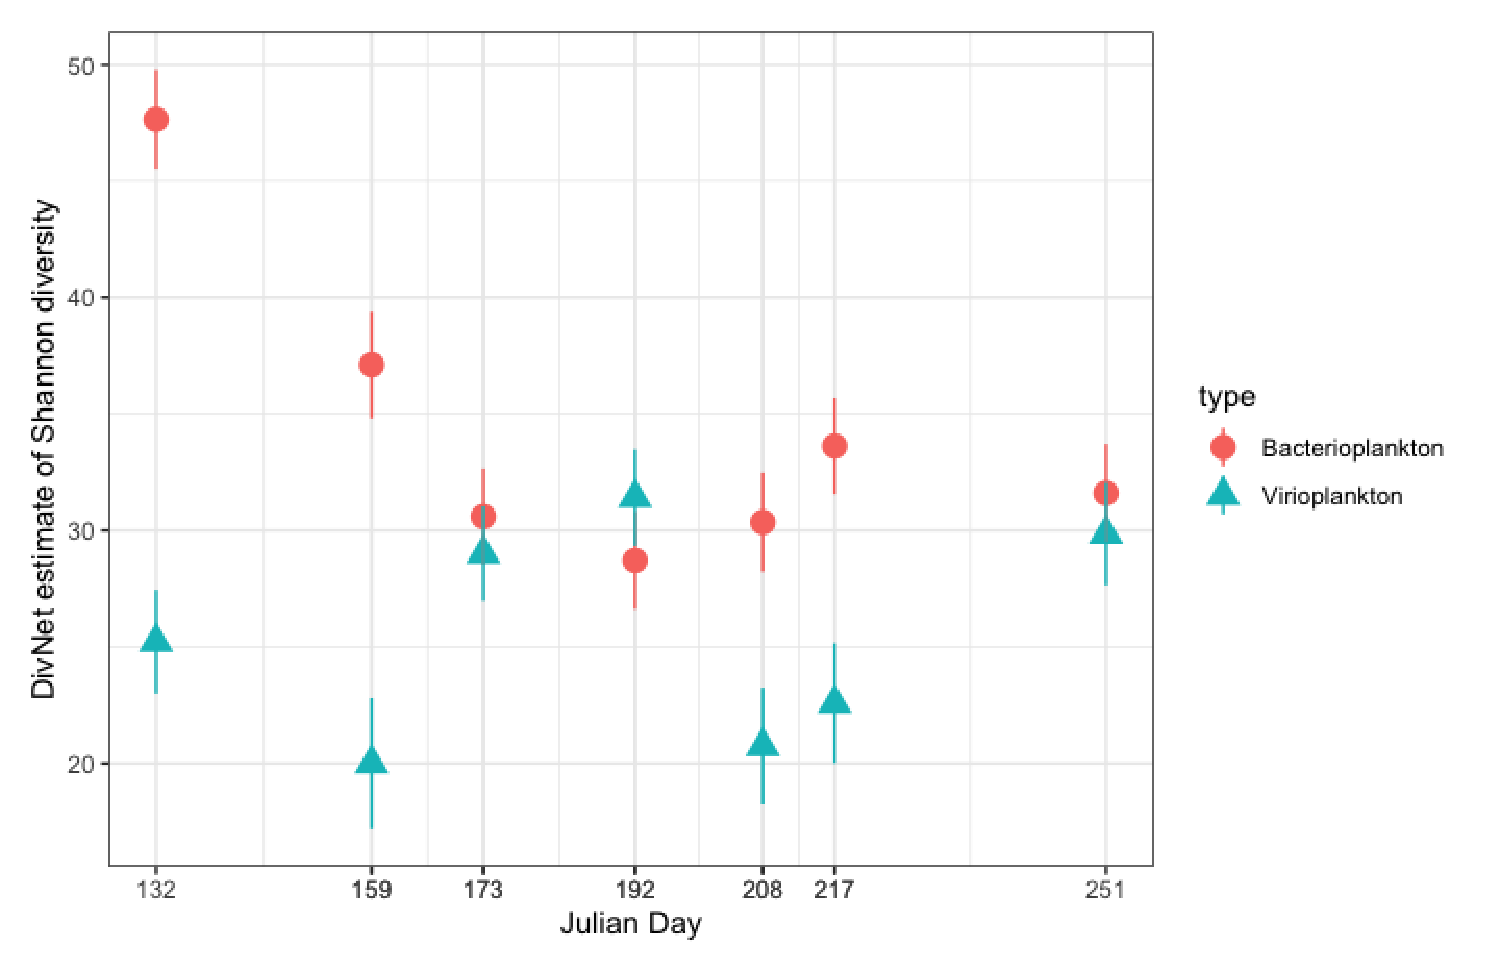
\includegraphics[width=15cm]{Bacterial_and_viral_shannon_day}
\end{center}
\caption{An Inverse Relationship was observed between estimated Shannon diversity of bacterioplankton (red) and virioplankton (cyan).
}
\label{alpha_div} 
\end{figure*}

Alpha diversity was computed for estimated Shannon diversity and tested for significance over time and over depth using DivNet. 
DivNet is a bioinformatics tool to estimate and compare ecosystem diversity across one of multiple environmental covariates and ignores the influence of other environmental covariates.
DivNet focuses on differences between ecosystems rather than differences between samples.
Thus, the hypothesis testing claims the the influence of certain environmental features to the diversities of communities.

An Inverse Relationship was observed between estimated Shannon diversity of  bacterioplankton and virioplankton (Figure~\ref{alpha_div}).
Bacterioplankton Shannon diversity experienced a local minimum on Jun22 (Julian Day 192), coinciding with the start of seawater stratification and nutrient depletion.
At the same time, virioplankton Shannon diversity experienced a local maximum. It is likely because that the dominant bacteria on Jun22 (Julian Day 192) had broad RTPR-carrying phage ranges.
A slight increase of bacterioplankton Shannon diversity was observed after Jun22, likely causing by regulation effects on phage infection. 
Phage are thought to play a crucial role in the maintainance and stabilization of diversity in natural bacterial communities.
The increase of bacterioplankton Shannon diversity decreased the virioplankton Shannon diversity in return as dominant bacteria having broad RTPR-carrying phage ranges were replaced with bacteria having narrower RTPR-carrying phage ranges.

\subsection{Correlations between Individual Bacterioplankton and Virioplankton Populations}

\begin{figure*}[t]
\begin{center}
\includegraphics[width=15cm]{within_fraction_proportionality}
\end{center}
\caption{
Proportionality test within (A) bacterioplankton and (B) virioplankton communities along sampling days at 50 m depth. Each panel represents clusters of concordant ASVs or OTUs with an expected 􏰄 value cutoff of 􏰀0.85 (bacterioplankton) or 0.65 (virioplankton). Each line in a cluster plot is the Loess line of best fit for the clr relative abundance (CLR Abundance on the y axis) of an individual ASV or OTU across sampling days (x axis). A 0 value indicates that the relative abundance of an ASV or OTU is equal to the mean log2 relative abundance of all ASVs or OTUs, while a positive or negative value indicates relative abundances greater or less than the mean log2 relative abundance, respectively. ASV lines of best fit are colored according to the class that the bacterioplankton ASV is classified into according to the key in (A). OTU lines of best fit are colored according to the clades that the virioplankton OTU is classified into according to the key in (B). Virioplankton clades are defined manually in the RTPR tree (C). Note that many of the clusters contain bacterioplankton ASVs related by the same class (A, C, D, E, G, H, I and L in (A)) and have approximately equal ratios between each other. And many of the clusters contain virioplankton OTUs related by the same clade (A, B and D in (B)) and have approximately equal ratios between each other as well. Associated bacterioplankton ASVs (A, C, D and F in (A)) related by different classes mostly had unequal ratios between each other along sampling days. 
}
\label{within_fraction_proportionality} 
\end{figure*}

we used an expected value of 􏰄metric to identify clusters of coassociated features (ASVs for bacterioplankton and OTUs for viroplankton) in the data set. 
This strength of association approach identifies features where both the direction and magnitude of variance are similar in the multidi- mensional data set. 
In a multivariate compositional sense, the metric is measuring both the slope of the correlation of the centered log ratio (clr)-transformed values and the correlation itself. 
A slope of 1 and a correlation of 1 are preferred. 
The 􏰄 metric coupled with a Bayesian estimation of feature relative abundance has the advantage of being agnostic to the level of sparsity in the data, unlike other recent approaches that depend on this sparsity.
ASVs from bacterioplankton had stronger association to each other than OTUs from virioplankton.
Each panel in \textbf{(A)} in \textbf{Figure~\ref{within_fraction_proportionality}} show the relative abundance of bacterioplankton ASVs assigned to one of 9 classes that had an expected 􏰄 value of 􏰀0.85, plotted against sampling day as a continuous variable. 
Each panel in \textbf{(B)} in \textbf{Figure~\ref{within_fraction_proportionality}} show the relative abundance of viroplankton OTUs assigned to one of 7 clades that had an expected 􏰄 value of 􏰀0.65, plotted against sampling day as a continuous variable.

This approach identified twelve distinct bacterioplankton clusters and four distinct virioplankton clusters, and many clusters contained ASVs classified into the same classes or OTUs classified into the same clades. 
And the ASVs related to the same classes or OTUs related to the same clades within the same clusters have approximately equal ratios between each other.
It is likely that the most strongly associated groups include predominantly members of the same phylogenetic groups because different members of the same phylogenetic groups have similar growth requirements, limitations, and interactions.
On contrast, associated ASVs from different phylogenetic groups mostly had unequal ratios between each other along sampling days.


\section{DISCUSSION}

\subsection{Environmental Changes Accompanying Temperature Changes Influence both Bacterioplankton and Virioplankton communities}

Place holder for oceanographic knowledge




\subsection{Seawater Stratification Influenced Bacterioplankton Diversity and Subsequently Influenced Changes in Virioplankton Diversity}
Seawater was well-mixed in the beginning of the sampling period (prior to June) as shown in Figure~\ref{watercolumn}.
Water stratification started in early June, suggesting a down-welling anticyclonic vortex (Figure~\ref{watercolumn}).
The downwelling vortex prevented nutrient from deeper and colder water from welling up to the sea surface, causing nutrient depletion. 
Water stratification continued throughout the summer and mitigated in early August, suggesting that seawater could well up and bring nutrient from bottom water to the surface to supply the nutrient.
Beta and alpha diversity of bacterioplankton and virioplankton communities changed with the changes of seawater characteristics.

Bacterioplankton samples taken before Jun22 are more similar to each other along PC1 but dissimilar to each other along PC2 (A in Figure~\ref{bata_div}). 
Bacterioplankton samples taken after Jun22 are more similar to each other along PC2 but dissimilar to each other along PC1.
Virioplankton samples showed similar patterns with bacterioplankton samples (B in Figure~\ref{bata_div}).
As seawater stratification started in early June, the similarity and dissimilarity patterns between samples of bacterioplankton and virioplankton communities were likely caused by the different seawater characteristics before and after the seawater stratification.
Bacterioplankton samples taken from 75 m depth are very similar to each other except for sample May12\textunderscore75m (A in Supplementary Figure S1). 
The distinction might caused by salinity or other covariate factors as temperature is homogenous across all sampling days at 75 m depth (A in Figure~\ref{watercolumn}) while salinity is low on May12 but similarly higher in other sampling days at 75 m depth (B in Figure~\ref{watercolumn}).
Overall, bacterioplankton samples taken from 75 m depth are similar to each other because seawater was mostly stable at 75 m depth compared to other sampling depths.
Bacterioplankton samples taken from 0 m and 5 m depth are highly dissimilar to each other, likely caused by the high disturbance on the sea surface along sampling days.
Virioplankton samples taken from different depths did not show clear patterns (B in Supplementary Figure S1), likely caused by two reasons: Firstly, viroplankton living in the sampling depths carried functionally similar RTPR as the environments are mostly stable in the pelagic oceans.
Secondly, RTPR, as a marker gene, does not provide as high resolution as the one provided by 16S rDNA provided because RTPR is a functional gene and not carried  by all viruses while 16S rDNA is a conserved phylogenetic gene carried by all bacteria.

Bacterioplankton Shannon diversity decreased from May12 (Julian Day 132) to Jul11 (Julian Day 192) as seawater stratification started and intensified.
It is likely because that down-welling anticyclonic vortex caused nutrient depletion at the surface seawater, subsequently caused less taxonomic groups of of bacteria surviving in the environment.
The existing dominant bacteria are likely to have broader phage ranges, as virioplankton Shannon diversity increased from Jun8 (Julian Day 159) to Jul11 (Julian Day 192).
As a result, bacterioplankton Shannon diversity experienced a local minimum while virioplankton Shannon diversity experienced a local maximum on Jul11 (Julian Day 192).
Later on, viral regulation effects increased bacterioplankton Shannon diversity. 
Virioplankton Shannon diversity decreased in return at the same time.
Overall, bacterioplankton and virioplankton Shannon diversity have a reverse relationship.


\subsection{Phylogenetically Similar Bacteria or Functionally Similar Viruses Exist in Similar Environments}

\subsection{CoDa Analysis Methods Produced More Reproducible Results Than Commonly Used Methods}

\section{CONCLUSION}

Text. Text. Text. Text. Text. Text. Text. Text. Text. Text. Text.
Text. Text. Text. Text. Text. Text. Text. Text. Text. Text. Text.
Text. Text. Text. Text. Text. Text. Text. Text. Text. Text. Text.
Text. Text. Text. Text. Text. Text. Text. Text. Text. Text. Text.
Text. Text. Text. Text. Text. Text. Text. Text. Text. Text. Text.
Text. Text. Text. Text. Text. Text. Text. Text. Text. Text. Text.
Text. Text. Text. Text. Text. Text. Text. Text. Text. Text. Text.
Text. Text. Text. Text. Text. Text. Text. Text. Text. Text. Text.
Text. Text. Text. Text. Text. Text. Text. Text. Text. Text. Text.
Text. Text. Text.


\section{ACKNOWLEDGEMENTS}

Text. Text. Text. Text. Text. Text. Text. Text. Text. Text. Text.
Text. Text. Text. Text.


\subsubsection{Conflict of interest statement.} None declared.
\newpage

\bibliographystyle{apalike}
\bibliography{reference}



\end{document}
